\section{Implementasjon}
\subsection{Beskrivelse av kode}
Siden programmet er bygd med Qt så er det enkelte filer og funksjoner som er definert på forhånd, altså disse må være her for at koden skal fungere. Dette gjelder for eksempel \textit{TCPClient.pro} og \textit{TCPClient.pro.user}. Selve designet til programmet ligger i \textit{TCPClient.ui} filen, og dette blir generert når jeg bruker Qt Designer og eksporterer designet til en lesbar fil.\\

Koden starter selvfølgelig med en main funksjon, hvor vi initialiserer objektet vårt og forteller Qt at vi ønsker å vise vinduet vårt.
\begin{lstlisting}
	#include <QApplication>
	#include "client.h"

	int main(int argc, char *argv[]){
		QApplication a(argc, argv);
		TCPClient client;
		client.show();

		return a.exec();
	}
\end{lstlisting}

Programmet har to header-filer, hvor vi har to forskjellige klasser. Hovedklassen som kjører selve Qt-vinduet er TCPClient, mens Socket-klassen blir brukt inne i TCPClient-klassen. I TCPClient-klassen er alle funksjonene relatert til klienten definert, mens i Socket-klassen er alle socket- og nettverksfunksjoner definert.
\begin{lstlisting}
	class TCPClient : public QMainWindow{
		Q_OBJECT

	public:
		explicit TCPClient(QWidget *parent = nullptr);
		~TCPClient();
		void addLog(QString);

	private slots:
		void on_connectButton_clicked();
		void on_clearButton_clicked();

	private:
		Ui::TCPClient *ui;
		Socket socket;
	};
\end{lstlisting}

\newpage
Det blir opprettet et objekt av Socket-klassen som er privat innenfor TCPClient-klassen, slik at vi får kjørt nettverksfunksjonene våre som ligger i Socket-klassen.
\begin{lstlisting}
	namespace Server{
		struct serverInfo{
			int sock, port;
			std::string ip;
			bool isConnected;
			sockaddr_in serv_addr;
		};

		struct studentInfo{
			char* number = new char[6];
		};

		enum MessageID{
			REQUEST_PORT = 0x01,
			RECEIVE_PORT = 0x02,
			PING = 0x03,
			PONG = 0x04,
			QUIT = 0x05
		};

		enum Errors{
			SOCKET_ERROR,
			INVALID_CONNECTION,
			INVALID_STUDNR,
			INVALID_PORTREQUEST,
			INVALID_PORTRESPONSE,
			PING_ERROR,
			PONG_ERROR
		};
	};

	class Socket{
	public:    
		Socket() : server{ 0, 0, "NULL", false } {}
		void makeConnection(std::string, int);
		void abortConnection();
		bool getConnectionStatus() const{ return server.isConnected; }
		char* getStudentNumber() const{ return student.number; }
		void verifyStudent(std::string);
		void requestPort();
		short receivePort();
		Server::MessageID portResponse();
		void pongServer();

	private:
		Server::serverInfo server;
		Server::studentInfo student;
	};
\end{lstlisting}

Alle funksjoner relatert til klienten ligger i \textit{client.cpp} filen, mens alle funksjoner relatert til socket ligger i \textit{socket.cpp}, slik at funksjonene er ryddig og lett å finne frem. I løpet av hele koden kjøres 7 funksjoner: makeConnection(), abortConnection(), verifyStudent(), requestPort(), receivePort(), portResponse(), pongServer().

\subsection{Demonstrasjon}
I figuren under er klienten koblet til serveren med riktig IP addresse, port og student nummer. Serveren vil da returnere en ny port som klienten må koble til, og deretter skal klienten holde en aktiv forbindelse ved å motta en ping og svare med pong inntil serveren sier stopp. Klienten er testet mot egen server som er programmert i Python med samme protokoller som Christians server.\\\\
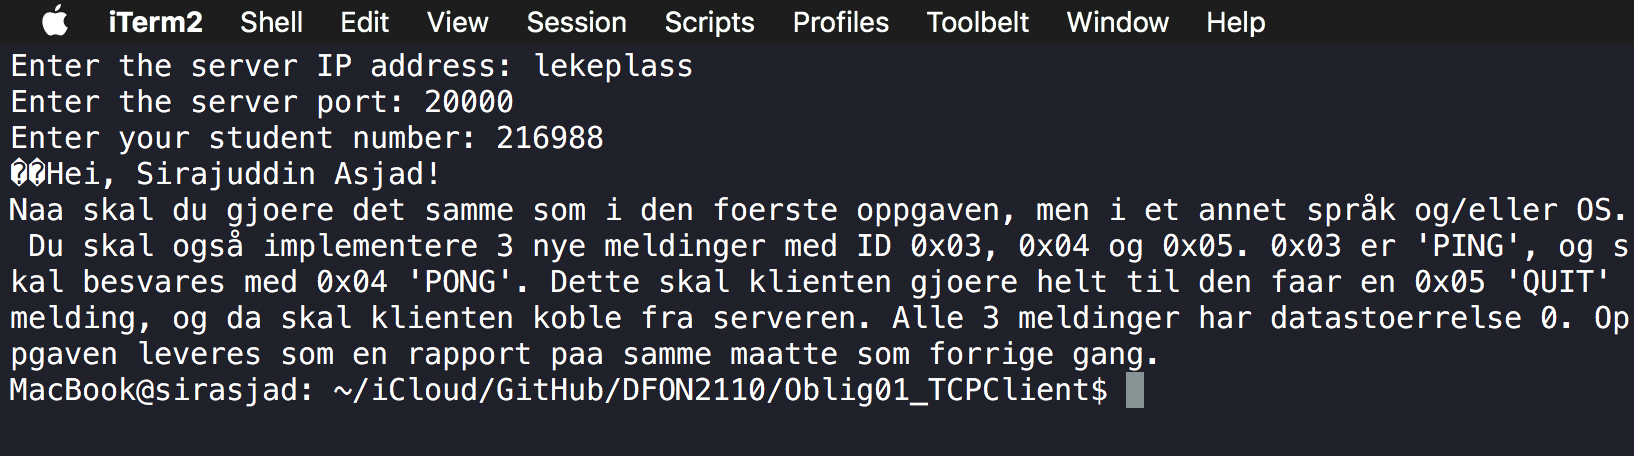
\includegraphics[width=\textwidth]{demo}
